% DIPOLOMARBEITS TABELLEN ENGLISCH ########################
\newpage
\begin{center}
\textbf{\LARGE DIPLOMA THESIS}

\textbf{Documentation}
\end{center}

\begin{tabular}{|p{53mm}|p{103mm}|@{}m{0cm}@{}}
\hline
\vspace{-0.11cm} Authors  \vspace{0.11cm} & 
\vspace{-0.11cm} Clemens Schlipfinger \newline Felix Schneider \vspace{0.11cm} & \\
\hline
\vspace{-0.11cm} Form \newline Academic year \vspace{0.11cm} & 
\vspace{-0.11cm} 5AHIT \newline 2023/24 \vspace{0.11cm} & \\
\hline
\vspace{-0.11cm} Topic \vspace{0.11cm} & 
\vspace{-0.11cm} Visualisation of the results of the electricity grid model \vspace{0.11cm} & \\
\hline
\vspace{-0.11cm} Co-operation partners \vspace{0.11cm} & 
\vspace{-0.11cm} Siemens AG Austria \vspace{0.11cm} & \\
\hline
\end{tabular}

\vspace{0.5cm}

\begin{tabular}{|p{53mm}|p{103mm}|}
\hline
\vspace{-0.11cm} Assignment of tasks \vspace{0.11cm} & 
\vspace{-0.11cm} Siemens is developing a new programme package for the real-time calculation of power grids. The quality of the network model is of the utmost importance for this calculation, but due to its size, errors are unavoidable. Currently, errors are stored in confusing log files. A fail-safe system with structured visualisation is required for simple evaluations. \vspace{0.11cm} \\
\hline
\end{tabular}

\vspace{0.5cm}

\begin{tabular}{|p{53mm}|p{103mm}|}
\hline
\vspace{-0.11cm} Realization \vspace{0.11cm} & 
\vspace{-0.11cm} The application uses the technologies \wordindoublequotes{Apache Kafka}, \wordindoublequotes{PostgreSQL} and the \wordindoublequotes{Java Spring}-Framework for the backend. The interface to the frontend has been implemented with \wordindoublequotes{GraphQL} and the frontend itself with \wordindoublequotes{Angular}. \vspace{0.11cm} \\
\hline
\end{tabular}

\vspace{0.5cm}

\begin{tabular}{| p{53mm}|p{103mm}|}
\hline
\vspace{-0.11cm} Results \vspace{0.11cm} & 
\vspace{-0.11cm} The project goal is to develop a user-friendly web application with filtering capabilities, graphs, and charts. This will involve utilizing a backend system that seamlessly integrates into the Siemens infrastructure by leveraging Apache Kafka, while ensuring the highest level of stability and fault tolerance. This will facilitate Siemens engineers in analyzing network model errors. \vspace{0.11cm} \\
\hline
\end{tabular}
\newpage

\begin{tabular}{|p{53mm}|p{103mm}|}
\hline
\vspace{-0.11cm} Architecture of the \newline application \vspace{0.11cm} &
\vspace{-0.11cm} 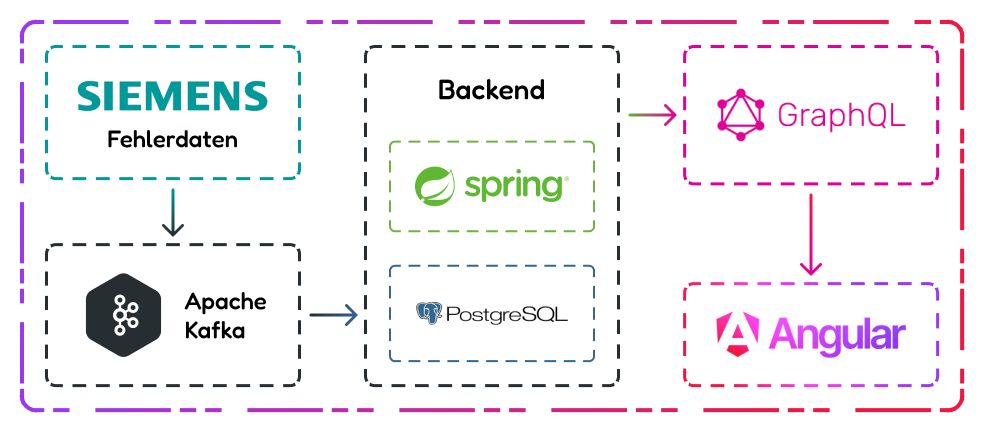
\includegraphics[width=0.62\textwidth]{content/img/Architecture/Architecture.jpg}
    This graphic shows the architecture of our prototype. The data comes from the Siemens GNA and is stored in the PostgreSQL database through Kafka. From there, it can be retrieved by the frontend via a GraphQL API. \vspace{0.11cm} \\
\hline
\end{tabular}

\vspace{0.5cm}

\begin{tabular}{|p{53mm}|p{103mm}|}
\hline
\vspace{-0.11cm} Participation in competitions Awards \vspace{0.11cm} &
\vspace{-0.11cm} Bosch Innovation Award 2024 \vspace{0.11cm} \\
\hline
\end{tabular}

\vspace{0.5cm}

\begin{tabular}{|p{53mm}|p{103mm}|}
\hline
\vspace{-0.11cm} Accessibility of diploma thesis \vspace{0.11cm} &
\vspace{-0.11cm} The written part of the work is publicly accessible. However, there is a blocking notice on the prototypes, as Siemens owns the copyright to the programme code. \vspace{0.11cm} \\
\hline
\end{tabular}

\vspace{0.5cm}

\begin{tabular}{|p{5.3cm}|p{4.93cm}|p{4.93cm}|@{}m{0cm}@{}}
\hline
\vspace{-0.11cm} Approval \newline (Date / Sign) \vspace{0.11cm} & 
\vspace{-0.11cm} Examiner \vspace{0.11cm} & 
\vspace{-0.11cm} Head of Department / \newline College \vspace{0.11cm} & \\ [4cm]
\hline
\end{tabular}